% Copyright (C) 2019 Cui Jialiang ( SESS, PKU )。 All rights reserved。

% TODO 添加中文参考文献
\newpage
\section{研究现状}
本节将介绍像素级视频影像跟踪算法及其相关算法的研究现状,为接下来介绍论文的理论创新铺垫基础。
\par
需要提前指出的是,本文所提出方法将是像素级别的处理技术在视频目标跟踪问题上的一个应用,并不是现在狭义上定义的视频目标跟踪算法\footnote{这个指生成矩形结果的视频目标跟踪算法}。但其中很多思想借鉴了现在的视频目标跟踪算法。因此在研究现状部分我们依然会着重分析视频目标跟踪算法,同时将介绍像素级别处理技术与深度学习思想。

\subsection{视频目标跟踪算法}
这里介绍的视频目标跟踪算法均是矩形级算法。视频目标跟踪是目前视频处理的一个很热门的研究方向。
\par
视频目标跟踪算法主要分为产生式模型和判别式模型。
\par
产生式模型指基于当前时刻及前一段时间的目标状态,结合新加入的帧的视频内容,直接根据概率模型产生一个新的跟踪目标。在计算能力极差的八九十年代,许多早期的模型
\supercite{schalkoff1982model}
都是产生式模型。直到20世纪初,产生式模型依然是主流。基于Kalman滤波的许多模型
\supercite{kim2002fast, weng2006video, comaniciu2003kernel}
都为推动跟踪效果做出过贡献。
\par
然而在现在\footnote{本文完成于2019年},判别式模型已经完全占据了视频目标跟踪的主流。2012年Hinton提出AlexNet 
\supercite{krizhevsky2012imagenet} 
后,深度学习这一划时代的思想迅速站上了图像处理界的主流。由于卷积神经网络
\supercite{krizhevsky2012imagenet} 
(Convolution neural network)在图像处理的普适性,在:
\begin{itemize}
    \item 图像分类\supercite{krizhevsky2012imagenet, witten2016data, he2016deep}
    \item 图像分割\supercite{long2015fully}
    \item 目标检测\supercite{ren2015faster, redmon2016you}
\end{itemize}
等领域均赢得了学界的认可,迅速与传统方法结合,成为这些研究方向必不可少的重要方法。
\par
在视频跟踪问题上,深度学习方法同样有较好的表现。经过几年发展,脱颖而出的许多基于深度学习的视频目标跟踪算法都是判别式模型。判别式模型指分两步完成跟踪的一种模型,第一步是利用提取特征的方法,将新帧作为一个图像做特征提取运算;第二步是结合提取出的特征和之前的跟踪结果,在提取出的特征中选择要跟踪的目标。具有代表性的有2016年的MDNet \supercite{nam2016mdnet}算法。该算法的主要思想是利用一个预先训练好的深度神经网络将送入的新帧作为图像提取特征,再形成多个次级网络进行目标跟踪。还有一些基于检测的目标跟踪,如ROLO\supercite{ning2016spatially}算法,先利用目标检测技术检测出很多目标,再从这些目标中选择一个和正在跟踪的目标比较像的目标作为跟踪结果。
\par
如前文所说,由于当今计算能力的爆发,能很快得到大量的目标检测结果,判别式模型大行其道。但判别式模型从思想上是目标检测的产物,其执行过程中将花费大量的时间去生成根本不是被跟踪目标的其他目标。本文将提出的是一种生成式模型,试图重新从目标跟踪的本质任务出发。

\subsection{像素级图像处理算法}
区别于典型的图像分类与目标外包框检测问题,像素级别(Pixel-wise)的图像处理需要获得一个覆盖全图的,精确到目标轮廓信息的结果。现在最常见的像素级别应用是图像分割。在图像分割领域,以早期的分水岭算法
\supercite{olsen1997multi}
为代表的传统阵营
\footnote{这里的传统阵营指用非神经网络方法的算法的处理方式}
已经有一系列研究。虽然分水岭算法有许多改进
\supercite{grau2004improved}
,但只能在大尺度图像上表现较好。对复杂情况下的分割效果依然不够智能。在深度学习技术出现后,深度学习很快就被运用于分割领域。最成功的典型是由U-Net
\supercite{ronneberger2015u}
开创的编码-解码模式。与之类似的还有SegNet
\supercite{badrinarayanan2017segnet}
将U-Net的升级模型稍加改动后得到了更好的效果。
\par
特别值得关注的是,纽约大学的Won-Dong Jang等于2017年提出过基于深度学习的实时视频分割算法\supercite{jang2017online}。但其并不是跟踪算法。
\par
但这些算法都是为图像分割设计的。相比与图像处理算法,视频处理算法更需要注意帧与帧之间的关系。上一段提到的著名的SegNet图像分割算法的演示阶段用的是视频数据做展示,但其只是将视频拆成了完全独立的图像进行处理,仔细观察会发现许多细节的处理会缺乏连贯性。

\subsection{像素级别视频目标跟踪算法}
近年来,像素级视频目标跟踪思路有少部分研究。
\par
美国学者Chad Aeschliman等在2010年提出过融合图像分割和目标跟踪的思路\supercite{aeschliman2010probabilistic}。德国学者Vasileios Belagiannis等在2012年提出过基于图像分割的目标跟踪算法\supercite{belagiannis2012segmentation}。韩国学者Jeany Son等在2015年提出过基于树模型的基于图像分割的目标跟踪算法\supercite{son2015tracking}。这些算法都借用了图像分割的算法思路,使用像素级别的数据训练分析,但最终输出依然是矩形级的结果。
\par
纽约大学的Yilin Song等在2017年完成的一项工作\supercite{DBLP:journals/corr/abs-1711-07377},该文用Conv-LSTM技术\supercite{PatrauceanHC16}尝试了对像素级别目标的视频目标跟踪。但该研究使用的手段复杂,最终结合了两个复杂的模型才得到结果(下一章\ref{section:pixel_wise_vot_2017_intro}中将介绍)。在更早的2007年,Hua等人用K-means算法也尝试过像素级别的跟踪\supercite{hua2008k},但由于没有结合深度学习算法,得到的结果也并不理想。
\par
本文希望提出的像素级别跟踪算法将建立在一个单独简洁的框架上,结合目前像素级别处理技术和目标跟踪技术的精髓,实现一个思路清晰的算法,并尝试寻求更好的结果。

\subsection{深度学习技术的发展}
2016年alphago\supercite{wang2016does}让许多人认识到了深度学习技术的能力。实际上更早之前深度学习研究工作就已经展开。
\par
2012年Hinton等人主导的深度学习技术能在图像处理,自然语言处理等方向大放异彩的主要原因之一,是深度学习采用了简单的模型,配合上高度自由可训练的参数,从而得到了更好的结果。简单的模型指CNN\footnote{Convolution Neural Network, 卷积神经网络},RNN\footnote{Recurrent Neural Network, 循环神经网络}等。前者主要用于处理空间尺度,即图像;后者主要处理时间尺度,即语音和视频。CNN和RNN的结构都很简单,由于权值共享思想,需要训练的参数也很少。但由于其采用了仿生学的原理,得到的结果往往比传统算法优秀。
\par
更早的,在20世纪末,就已经有人提出并用图像数据尝试了深度学习\supercite{lecun1998gradient}。但直到近年来,GPU计算的普及才使得深度学习技术有了更大的用武之地。
\par
本文提出的算法将主要采用深度学习方法,力求用一个简单的深度学习模型解决复杂的问题。

\par
2013年,加州大学伯克利分校的发布了Caffe\supercite{jia2014caffe}深度学习工具(后来与PyTorch\supercite{paszke2017automatic}合并),谷歌公司于2017年初发布Tensorflow\supercite{abadi2016tensorflow}的python版本API。在国内,百度也发布过自己的深度学习框架PaddlePaddle\supercite{recognize_digits_paddle}。
\par
这些开源免费,高效实用,简单易用的工具使深度学习算法的实现变得十分容易,增加了个人开发者对深度学习算法贡献的容易度。

\subsection{视频跟踪数据集}
近年来随着研究的火热,产生了许多网络上共享的数据集,典型的有2009年的ImageNet\supercite{imagenet_cvpr09}。
由于深度学习需要大量的训练数据,开放的数据集直接推动了深度学习的发展。
\par
在跟踪领域最典型的有VOT\supercite{VOT_TPAMI}和OTB\supercite{WuLimYang13}数据集。特别是VOT数据集2016年的像素级别数据\supercite{Vojir-TR-2017-01},以人工标注的方式提供了像素级别的视频跟踪训练集。在图像分割问题上同样有许多数据集,如VOS\supercite{Cae+17}等。这些数据集的数据量很大,数据质量也很好,给模型训练带来了许多方便。本文将直接使用VOT等跟踪数据集,并尝试过使用一些分割数据集对模型进行更为细节的训练。

\newpage
\section{论文主要研究内容与结构安排}
论文主要先进行了综述调查,发现了问题,总结了前人的研究结果。提出了一种基于CNN和RNN的像素级跟踪算法,并对这种算法进行了结构调优。论文还实现了该算法,并对结果进行了定量分析。

\begin{figure}[htbp!]
    \centering
    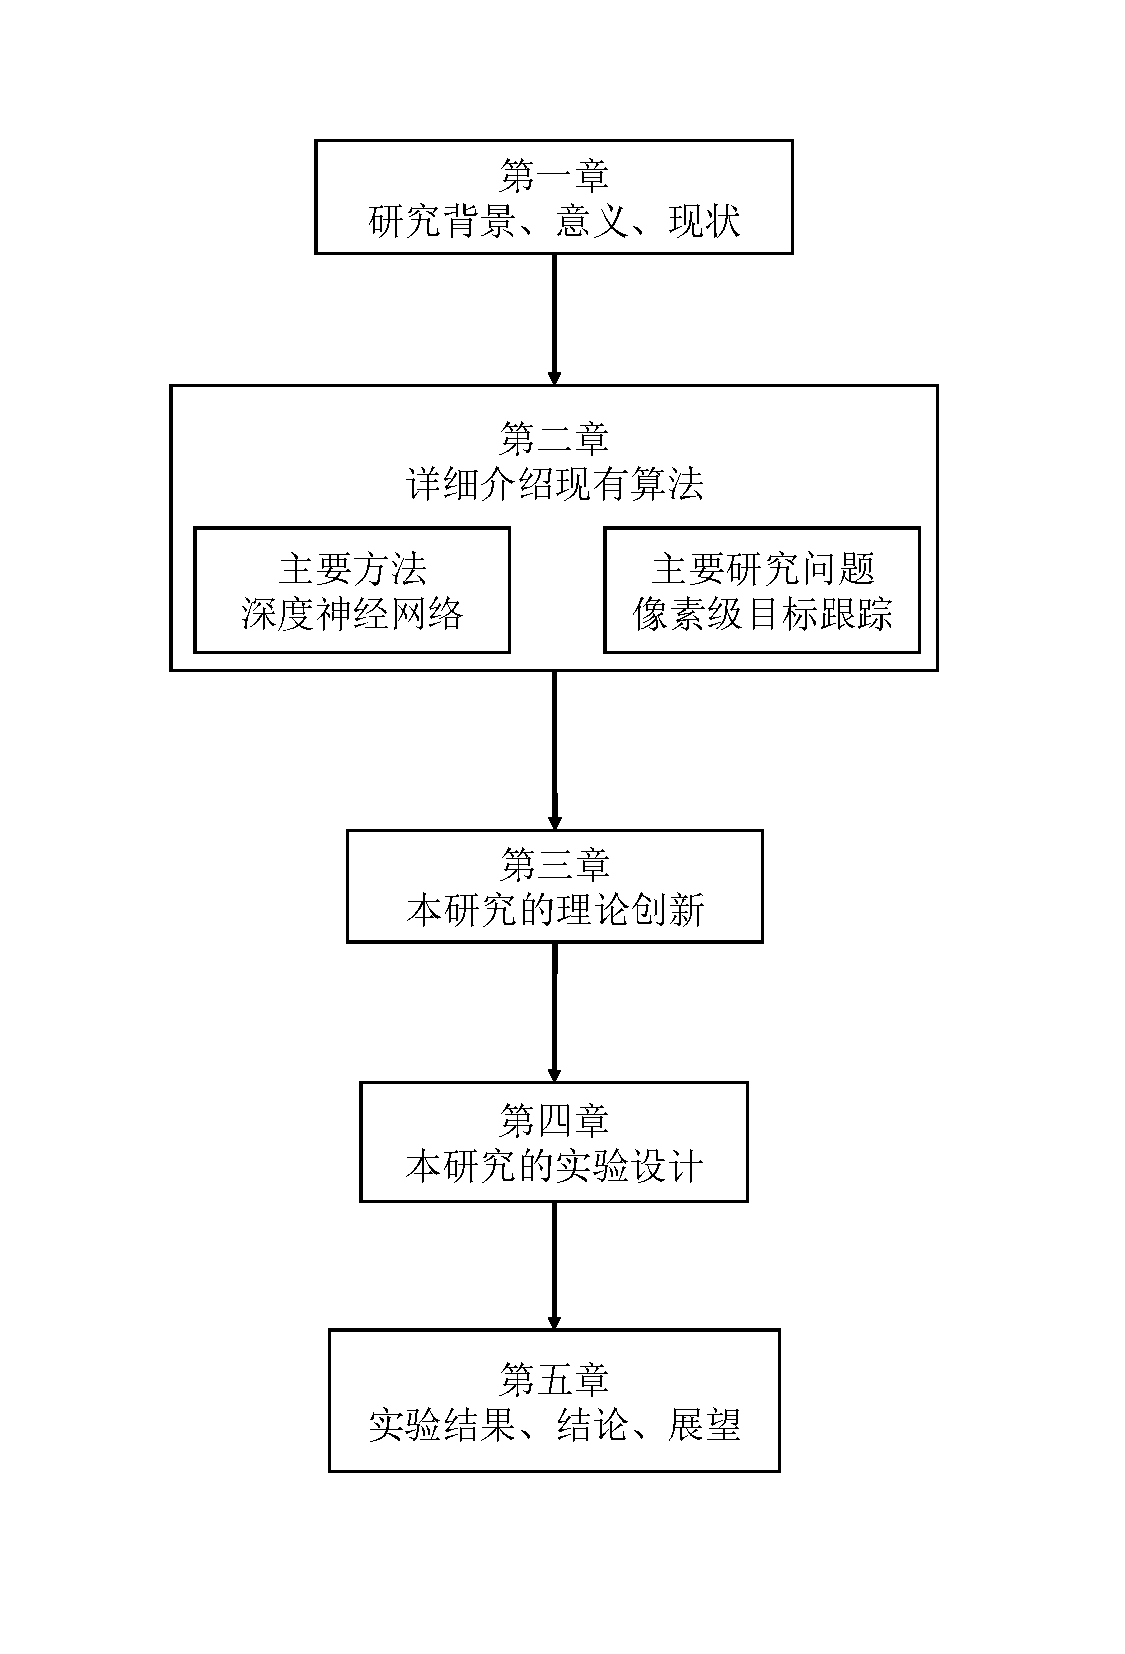
\includegraphics[width = 1.\textwidth]{chap/img/thesis_structure.pdf}
    \caption{
        论文结构图
        }\label{fig:thesis_structure2}
\end{figure}
\par
本论文的结构安排大致如图\ref{fig:thesis_structure2}所示。